\section{Primary Research Survey}
\label{research:PrimaryResearchSurvey}
When creating this survey I heavily utilised my prior research in addition to my prior experience filling out forms. I wanted to achieve around 30 responses to gather a large enough data pool that I could analyse for trends. 

Whilst Written response style questions can provide much more in-depth user data I've found that these can be time consuming / frustrating to complete and therefore should be used in moderation to ensure a high user completion rate - I would rather a potential respondent answered a couple of checkbox questions successfully then saw a typed response and clicked off the survey thus submitting no information.

I've also found that too many mandatory questions can be frustrating especially when I have nothing to say for a certain part. With this in mind I am choosing to make each question optional to answer, whilst this does mean a resonant could complete the form with only one question I am hoping this will be a minority and this change will improve the completion rate of my form.

 the key data I wanted to gain was:
 \begin{itemize}
    \item How often people take notes 
    \item Which devices and methods they use
    \item  If they have any preexisting ideas about why current software provisions aren't ideal
    \item How people find their notes
    \item Any feedback / tips they would have for me
 \end{itemize}
	
And additionally a smart amount of identifying information such as their profession (useful to compare students vs professionals etc) and optionally, their email if they wish to hear more about the project In the future - this sets me up to ask for feedback once I have a functioning minimum viable product that I am ready to share.

After completing my form I asked my parents (who both have extensive experience in marketing and consumer research) for their opinions on the questions I was asking. Whilst they liked the tone and style of the questionnaire they had some constructive criticism to help further improve the data I will collect:

\begin{tabularx}{\textwidth}{
  >{\raggedright\arraybackslash}X
  >{\raggedright\arraybackslash}X
  >{\raggedright\arraybackslash}X
  >{\raggedright\arraybackslash}X
}
\toprule
\textbf{Feedback} & \textbf{Purpose} & \textbf{Implemented} & \textbf{comment} \\
\midrule

suggested some slight modifications to the user categories I had posed & to further contextualise their opinions & \ding{51} & I added some new categories (Creative professional \& technology professional) and made It possible to select multiple categories 
 \\

 Updating note frequency question & Make wording clearer and interpretation more equal among participants & \ding{51} & Phrased question as being about note taking opportunities not just when people take notes \\

 Rephrase application category for generic note app & Make that option more understandable for less digitally versed participants & \ding{51} & Rephrased as device default note app (rather than purely using examples)
\\

Randomising order of "rank high to low" style questions & Make data more reliable rather than potentially creating bias with preset order (even if not intentional) & \ding{51} & \\


\bottomrule
\end{tabularx}

\subsection*{Updated Survey:}
\begin{figure}[H]
\centering
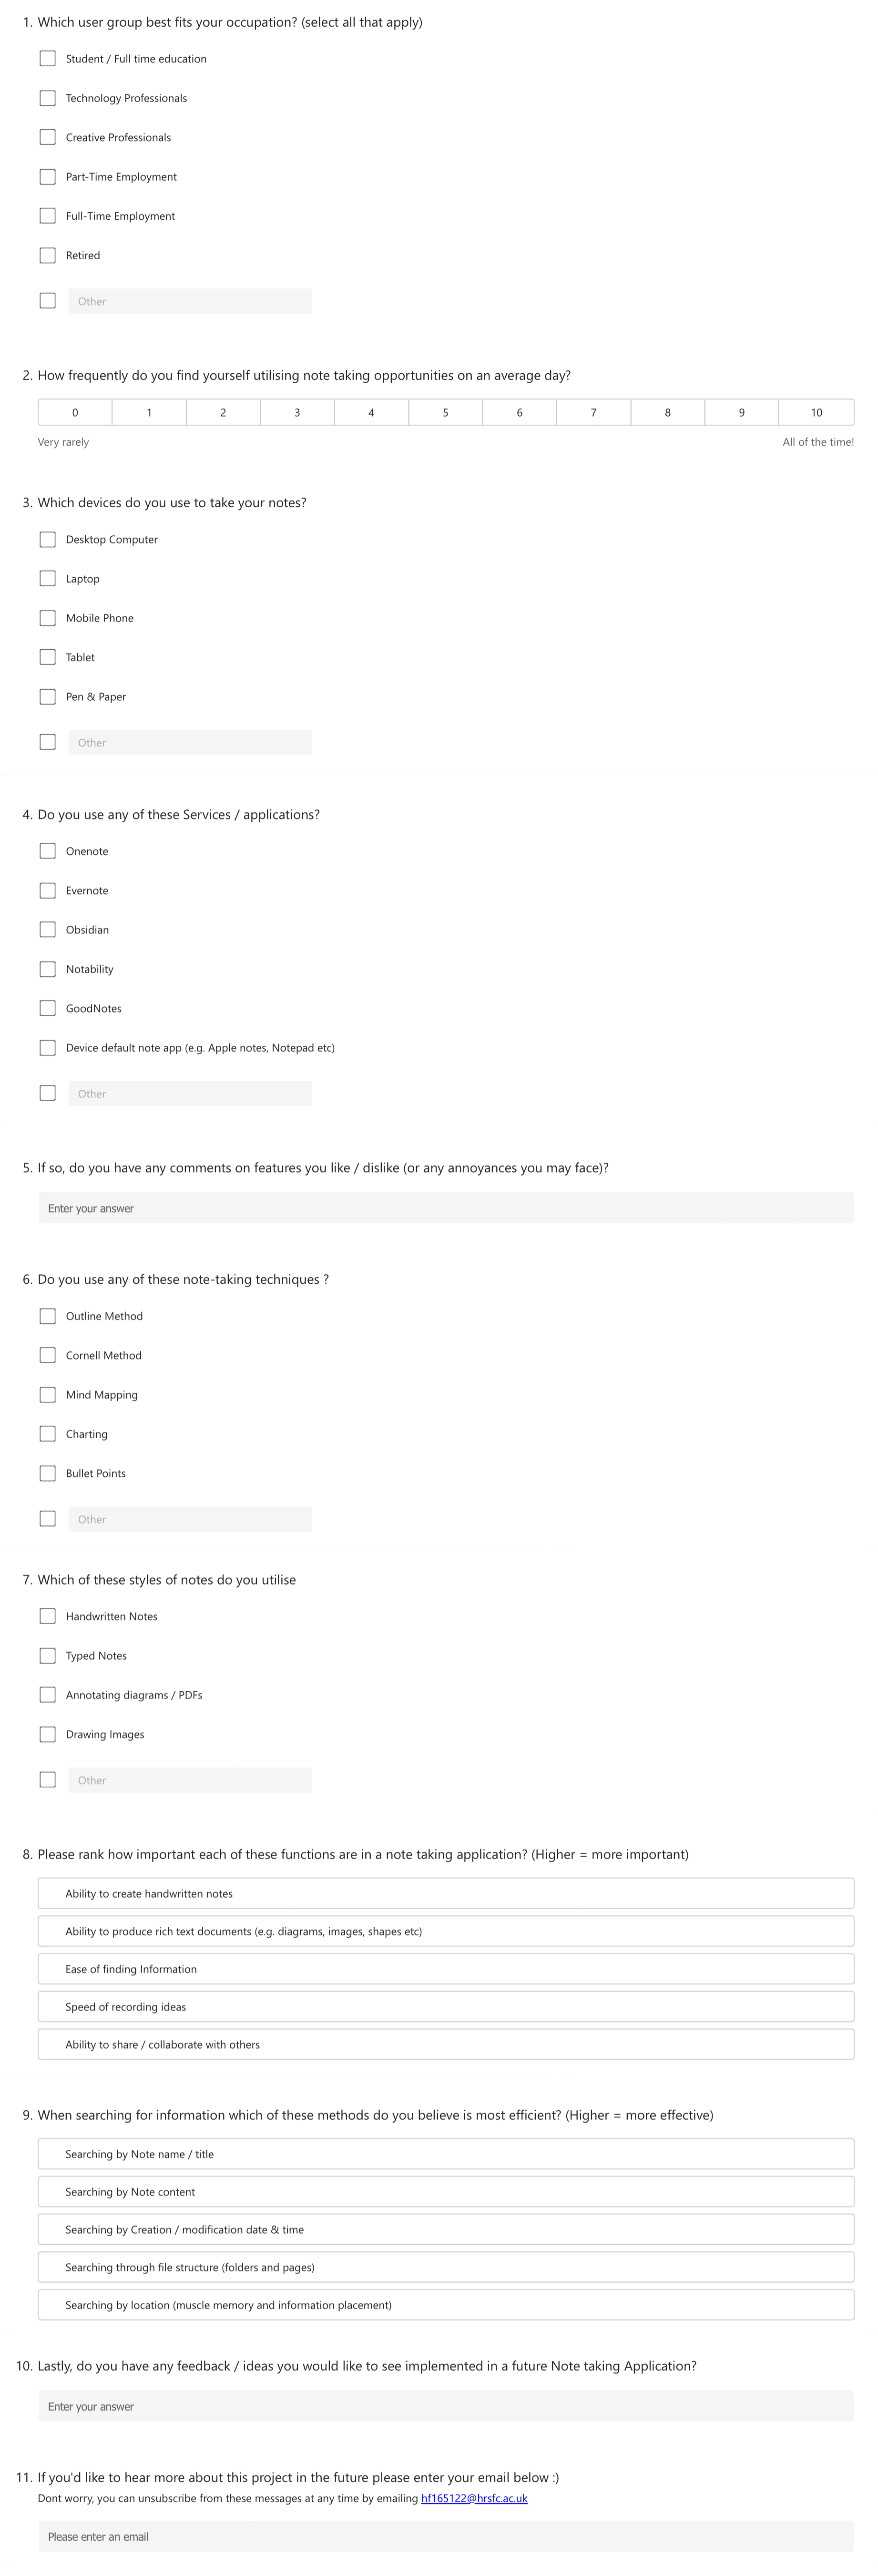
\includegraphics[width=0.5\textwidth]{Research/13_PrimaryResearchSurvey/media/questions.png}
\caption{Finalised Survey Questions}
\end{figure}